% Created 2019-07-14 Sun 12:17
% Intended LaTeX compiler: pdflatex
\documentclass[11pt]{article}
\usepackage[utf8x]{inputenc}
\usepackage[T1]{fontenc}
\usepackage{graphicx}
\usepackage{grffile}
\usepackage{longtable}
\usepackage{wrapfig}
\usepackage{rotating}
\usepackage[normalem]{ulem}
\usepackage{amsmath}
\usepackage{textcomp}
\usepackage{amssymb}
\usepackage{capt-of}
\usepackage{hyperref}
\setlength\parindent{0pt}
\setlength\parindent{0pt}
\usepackage{placeins}
\date{\today}
\title{Mémoire}
\hypersetup{
 pdfauthor={},
 pdftitle={Mémoire},
 pdfkeywords={},
 pdfsubject={},
 pdfcreator={Emacs 26.2 (Org mode 9.1.9)}, 
 pdflang={English}}
\begin{document}

\maketitle
\tableofcontents


\section{Sportagraph}
\label{sec:org595660f}
Sportagraph est une start-up filiale de Everspeed, fondée en 2013 et lancée en 2016 après trois années de recherche et développement (R\&D).
Son produit est un DAM (Digital Asset Manager) spéecialisé dans les événements sportifs.

Le DAM permet aux utilisateurs de stocker et de gérer plusieurs types de fichiers (principalement des images, mais les vidéos et d’autres types sont aussi supportés). 
L’équipe travaillant sur ce projet est composée de :
\begin{itemize}
\item Alex Macris : Chief Experience Officer
\item Edouard Binchet : Chief Strategy and Operation Officer
\item Régis Jean-Gilles : Lead Server Developer (mon tuteur d'alternance)
\item Benoit Hozjan : SaaS operation manager
\item Francois Jacquier : Lead Developer Front
\item Khedidja Almherabet : Développeur front-end
\item Mate Gyomrei : Développeur front-end
\item Daniel Denke : Développeur iOS
\item Zoltan Tarsoly : Test Automation Engineer
\item Youva Ammaouche : Assistant chef de projet
\item Stéphane : Développeur front-end
\item Ashant : Développeur front-end
\end{itemize}

En tant que développeur back end, je suis chargé de rajouter de nouvelles fonctionnalitées au DAM.
L'une des missions qui m'a été affecté est la détection des replays dans les vidéos de sport.
Cette fonctionnalité nous permettra de fournir à nos clients un résumé automatique des vidéos qu'ils uploadent sur le DAM.

\section{Introduction}
\label{sec:org6abe3fa}

Au cours des dernières années, les techniques d'apprentissage automatique ont joué un rôle de plus en plus important dans les systèmes de reconnaissance automatique.
Les avancements dans le domaine de l'apprentissage profond et l'accès à un volume massif de données ont permi de mettre en place des solutions de plus en plus performantes.
En particulier, l'adoption globale des téléphones intelligents et de leur caméra intégrée a accru de manière exponentielle le nombre de vidéos disponibles sur Internet, à tel point qu'il est devenu impossible pour l'humain d'ingérer manuellement le contenu de toutes les vidéos disponibles sur la toile.
Dans cet étude, nous allons nous intéressons à la tâche de "video summarization" ou, en français, de récapitulation de vidéo.
Plus particulièrement, nous focalisons notre recherche sur les vidéos de match de football.
Dans ces vidéos, notre objectif va être de parvenir à identifier les replays; car à partir de ces replays, nous serons capables de mettre en avant les moments importants du match.

\textbf{Pourquoi les replays ?} Un replay est la retransmission d'une action qui s'est déjà passé au cours d'une vidéo.
Les replays sont intéressants car ils sont un indicateur d'un moment fort dans une vidéo.
En effet, c'est l'équipe technique chargée du montage de la vidéo qui décide ou non de créer un replay pour une action, un replay est une annotation humaine sur une vidéo.
Typiquement, un replay sera incrusté dans la vidéo après une action importante comme, par exemple, un but ou un pénaltie.

\textbf{Caractéristique des replays} Les replays sont introduits et se terminent par un logo (\cite{Hao_Pan_2002}).
Ces logos ont en général une apparence qui se démarque facilement des autres images dans la vidéo.
Les replays ne sont pas à confondre avec les ralentis.
Les ralentis sont un type particulier de replays où l'action est montrée de nouveau en \emph{slow-motion}, mais tous les replays ne sont pas des ralentis.
C'est pourquoi, la vitesse de déplacement des objets dans l'image (pour détecter l'effet de \emph{slow-motion}) n'est pas un bon critère pour la détection de replay.

L'objectif de notre recherche est double.
Dans un premier temps, nous mettons en place un système de détection de replays en utilisant uniquement les méthodes "classiques" tels que ORB (\textbf{ref})
Ensuite, nous comparons plusieurs approches d'apprentissage automatique pour la tâche de détection dans les vidéos.
Enfin, nous comparons l'efficacité des méthodes de vision par ordinateur "classique" aux méthodes par apprentissage profond (deep learning).


\section{Détection des replays avec des approches "classiques"}
\label{sec:org33b8082}
L'un des objectifs de notre recherche est de mettre en place un modèle de détection de replays n'utilisant que des techniques ne faisant pas intervenir d'apprentissage automatique.
Ce modèle servira de base de comparaison avec le modèle par apprentissage automatique que nous proposerons par la suite.
Afin d'avoir le meilleur modèle, nous avons comparé plusieurs approches.

\subsection{A Robust Replay Detection}
\label{sec:org6c3ec95}
Cette approche détecte les replays en trouvant les logos dans la vidéo.
Les logos sont trouvés grâce à la luminance. Nous savons qu'un logo est présent pendant 0.8 secondes soit 18 frames pour une vidéo de 24 FPS.
Tous les frames qui ont obtenu un score supérieur à un certain seuil sont considérés comme des "logo templates".

\subsubsection{Calcul du score de la luminance et filtrage des frames}
\label{sec:org4af5348}
L'idée est de parcourir toute la vidéo et de calculer pour chaque frame la différence de luminance qu'il y a entre ce frame et les 17 frames précédents.
Nous obtenons un score L\(_{\text{i}}\) pour chaque frame i dans la vidéo.
Tous les frames dont le score est inférieur à un certain seuil sont écartés, les autres vont servir à trouver le logo template.

\subsubsection{Recherche du logo template parmis les frames filtrés}
\label{sec:org97046bd}
Le logo template est le frame qui représente le mieux tous les logos dans la vidéo.
Pour déterminer le logo template parmis les frames filtrés, l'algorithme K-means est utilisé pour séparer cet ensemble en deux (K = 2) en fonction de la luminance moyenne des frames.
Pour trouver le logo template, nous allons chercher dans le cluster avec le centre de cluster le plus élevé, puis sélection le frame m minimisant la distance avec tous les autres frames du cluster.

\begin{figure}[htbp]
\centering
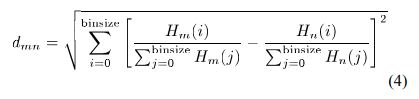
\includegraphics[width=10cm]{robust_calc_dist.JPG}
\caption{Formule de la distance entre deux frame dans le cluster \label{calc-dist}}
\end{figure}


\subsubsection{Recherche des logo}
\label{sec:org518b39d}
Une fois que le logo template est déterminé, chaque logo trouvé en 1 va être comparé avec le logo template.
La mesure de comparaison est la distance (équation 4) qu'il y a entre le frame et le template dans le cluster.
Tous les frames qui ont une distance inférieure à un certain threshold sont considérés comme des logos.

\subsubsection{Recherche des replays}
\label{sec:org2c6f744}
Une fois que les logos sont détectés, nous pouvons trouver les replays en cherchant les paires de logos éloignés de moins de 80 seconde (durée maximum d'un replay).

\subsubsection{Résultats obtenus et conclusion sur cette méthode}
\label{sec:org29fccb7}
\begin{center}
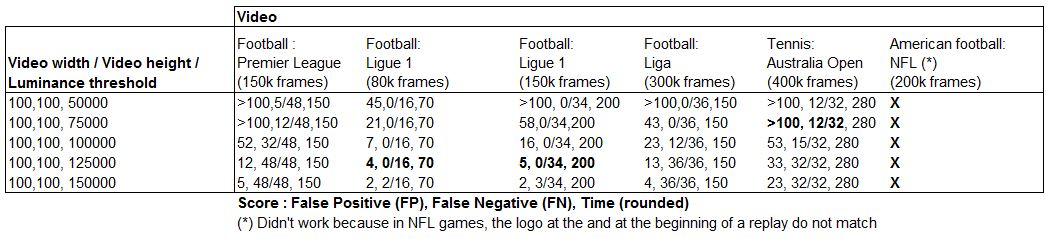
\includegraphics[width=15cm]{robust_res.JPG}
\end{center}
Après avoir implémenté cette méthode, nous avons constaté que celle-ci n'est pas efficace et ne fonctionne pas du tout sur notre ensemble de test.
Cette approche est trop dépendant de la luminance et elle ne parvient pas à détecter les logos peu lumineux.
De plus, les bases mathématiques (notamment la manière de choisir le cluster et la mesure de distance) sont un peu douteuses.
Enfin, celle-ci dépend trop du paramètre "seuil de luminance" affectant les logos détectés.
Le seuil de luminance fournis par les auteurs ne produit pas de bons résultats sur toutes les vidéos.
Nous n'avons pas réussi à trouver une valeur pour le seuil de luminance qui obtienne universellemnt de bons résultats.
Un seuil à 100000 détecte les logos de Ligue 1 mais pas les logos de Liga.
Un seuil de 75000 détecte les logos de Liga et de Ligue 1, mais laisse passer trop de faux positifs.
Les logos de Premier League quant à eux ne sont pas tous détectés avec un seuil à 50000, alors que ce seuil accepte un grand nombre de faux positifs.
Pour conclure, cette approche n'est pas celle qui va nous permettre de mettre en place un système de détection de replays robuste et efficace.

\subsection{Automatic summarization of soccer highlights using audio-visual descriptors}
\label{sec:orgd0f40e0}
Cette approche ressemble à la précédente, mais introduit néanmoins une différence importante : un pré-traitement sur la vidéo pour en extraire les plans.
\subsubsection{Algorithme}
\label{sec:org71b99fd}
\begin{verbatim}
S = Détecter tous les shots (plans) dans la vidéo
L = Pour chaque shot S_i:
1. L_i_start = La "luminance" des frames au début du shot
2. L_i_end = La "luminance" des frames à la fin du shot
3. L_template = Trouver le "logo template" dans L
4. Pour chaque logo l dans L:
   1. Diff l avec L_template = conversion grayscale puis somme de la soustraction pixel par pixel
   2. Si Diff l avec L_template < threshold => l est un logo
\end{verbatim}

\subsubsection{Conclusion}
\label{sec:org69547ef}
Cette méthode est trop semblable à l’approche “Robust Replay Detection” qui ne répond pas à nos besoin,
cette approche ne fonctionnera pas dans notre cas (la luminance n’est pas un critère assez discriminant pour la reconnaissance de logo).
Néanmoins, l’idée de découper la vidéo en “shot” (en plan) est intéressante et nous nous en servons par la suite.

\section{Les approches proposées}
\label{sec:orgbedc381}
Les méthodes "état de l'art" ne donnent pas d'assez bons résultats et ne peuvent pas être mises en production. 
Nous cherchons donc notre propre méthode.

Pour détecter les replays, nous faisons les hypothèses que :
\begin{itemize}
\item un replay a un logo de début (I)
\item un replay a un logo de fin (II)
\item les logos de début et de fin sont les mêmes (III)
\item les logos ont une forme facilement reconnaissable qui se distingue des  autres images dans la vidéo (IV)
\item un replay dure entre 2 et 90 secondes (V)
\end{itemize}

Nous proposons plusieurs approches permettant de détecter les logo de replay dans les vidéo de sport. 
Dans cette partie, chacune de ces approches n'utilisent que des algorithmes de computer vision classique (flouttage, filtre de Canny, ORB, \ldots{}) et des algorithmes de machine learning non-supervisés (K-NN).
Ces restrictions s'appliquent pour les raisons suivantes :
\begin{itemize}
\item le programme doit être le plus rapide possible (les réseaux de neurones sont en général trop lents, trop exigeant en ressource); d'où le choix d'algorithme plus simple.
\item si la solution doit être mise en production, il est préférable de ne pas avoir d'ensemble d'apprentissage à obtenir ou maintenir; d'où le choix d'algorithme non-supervisé uniquement.
\end{itemize}

\subsection{Détection des plans}
\label{sec:orgbc5136b}
Les approches que nous proposons itérent sur tous les frames de la vidéo, à la recherche des logo pouvant se trouver au début et à la fin des replays.
Si nous faisons l'hypothèse qu'un replay entraînera toujours un changement de plan, alors au lieu de rechercher les logo parmi tous les frames de la vidéo, nous réduisons la recherche à tous les frames qui sont entre deux plans.

\subsubsection{Online, Simultaneous Shot Boundary Detection And Key Frame Extraction For Sports Videos Using Rank Tracing}
\label{sec:orgaa8ca87}
Cette méthode est proposée par W. Abd-Almageed en 2008.

Chaque frame est converti en HSV et les histogrammes H, S et V sont calculés.
Un vecteur est formé pour chaque frame à partir de ces histogrammes.
Ensuite, une matrice M de dimension N * L, représentant une fenêtre de N frames va être formée à partir de ces vecteurs, où L est la taille des histogrammes et N la taille de la fenêtre.

L'algorithme SVD (singular value decomposition) va être appliquée sur M. M = UWV, où W est la matrice de valeur singulière.

Les diagonales de la matrice W comportent des poids S ordonnées de manière non croissante.
Le premier poid S\(_{\text{1}}\) est le poid maximal. Ces poids représentent l'information contenu dans le vecteur V.

Nous allons assigner un rang à la matrice M,  ce rang va être égal au nombre d'élement s dans S tel que s/S1 > threshold. Le rang va être calculé pour chaque fenêtre de frame dans la vidéo.

Si le rang d'une fenêtre est plus que grand que le rang de la fenêtre avant elle, alors le contenu visuel de la fenêtre est différent de la fenêtre précédente.
À l'inverse, si le rang est inférieure à la fenêtre précédente, alors le contenu visuel se stabilise. S'il est de 1, alors c'est stable.

Le début d'un frame est celui qui maximise le rang parmis les fenêtres environnantes.

\begin{enumerate}
\item Résultats obtenus et conclusion
\label{sec:orgaa983a5}
Cette méthode pour trouver les plans dans une vidéo est très efficace, et constitue la base de la suite de notre recherche.

En effet, avant de segmenter la vidéo en plan, nous comparions  N frames , où N peut être aussi grand que 400000 (pour des vidéo de 120 minutes à 60 fps).
Il est impensable d’utiliser un algorithme en O(N²), par exemple en comparant toutes les frames entre elles, avec un N aussi grand.

Après avoir segmenter la vidéo en plan, nous obtenons un N’ au alentours de 2000 pour une vidéo de 120 minutes à 60 fps. 
Nous pouvons donc nous permettre d’utiliser des algorithmes plus complexes que sans la segmentation en plan.
De plus, la segmentation en plan réduit le champs de recherche des frames logo, et donc le nombre de faux positifs potentiels.
\end{enumerate}

\subsection{Première approche : ORB}
\label{sec:orgba96dad}
Dans cette approche, nous cherchons à reconnaître les logo dans la vidéo.
Pour ce faire, nous optons pour une approche de clustering. L'idée est de clusteriser la vidéo en deux groupe : un groupe pour les frames logo, et un autre groupe pour les frames non-logo.

\subsubsection{Extraction des caractéristiques}
\label{sec:orgd2b999a}
OpenCV permet d'extraire des features à partir des images (détection des bords des objets dans l'image).
A partir de ça, nous pouvons représenter l'image comme un vecteur de feature.
Les méthodes d'extraction sont ORB et AKAZE.

\subsubsection{KMeans}
\label{sec:org2afbd08}
OpenCV implémente aussi l'algorithme KMeans. Celui-ci permet de regrouper les objets similaires en fonction de leur feature. 
Dans notre cas, il va nous permettre de créer 2 groupes d'images : logo / non logo.
L'avantage de KMeans est qu'il est est très rapide et assez efficace dans la plupart des cas.
C'est l'un des algorithmes de clusterisation les plus utilisés.

\subsubsection{Expérimentation et résultat:}
\label{sec:org15946e5}
Ensemble de test : une vidéo de ligue 1, une vidéo de liga, une vidéo de premier league et une vidéo NFL.
Dans toutes les expérimentations, la vidéo est découpée en shot (plan).
Soit S l'ensemble des shots.

\subsubsection{1 frame par shot}
\label{sec:org902acaa}
\begin{center}
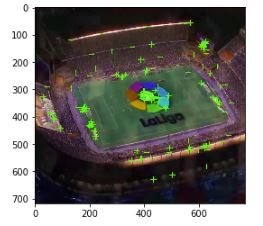
\includegraphics[width=.9\linewidth]{orb_simple_res.JPG}
\end{center}
\begin{verbatim}
- Récupérer le frame à la fin de chaque shot
  - nous obtenons |S| frame
- Pour chaque frame, calculer ses features (orb ou akaze)
  - Nous obtenons |S| vecteurs
- Utiliser KMeans avec K=2 pour séparer les vecteurs en deux groupes
  - le groupe le plus petit est le groupe des logo
\end{verbatim}

Résultats :
\subsubsection{{\bfseries\sffamily TODO} meilleurs res}
\label{sec:orgfe87627}
Mauvais sur toutes les vidéos

\subsubsection{W frames par shot:}
\label{sec:orga29ce9f}
\begin{verbatim}
- Récupérer W frames pour chaque shot
  - nous obtenons |S*W| frame, où W est le nombre de frame
- Pour chaque frame, calculer ses features (orb ou akaze)
  - nous obtenons |S*W| vecteurs
- Utiliser KMeans avec K=2 pour séparer les vecteurs en deux groupes
  - le groupe le plus petit est le groupe des logo
\end{verbatim}

Résultats :
Mauvais sur toutes les vidéos

\subsubsection{1 fenêtre de frame par shot:}
\label{sec:orgeef12ab}
\begin{center}
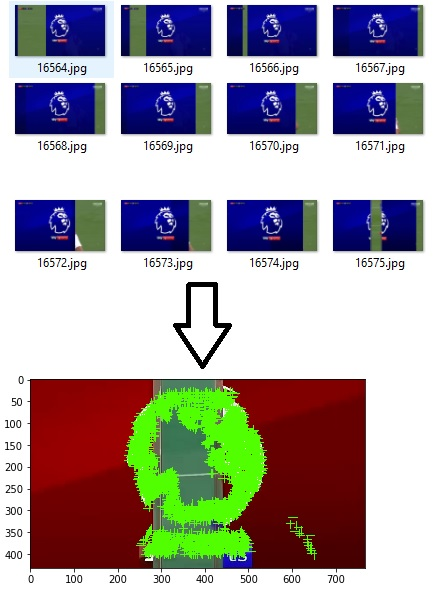
\includegraphics[width=.9\linewidth]{akaze_window_res.JPG}
\end{center}
\begin{verbatim}
- Récupérer W frames pour chaque shot, les régrouper en une fenêtre
  - nous obtenons |S| fenêtre de dimension W, où W est le nombre de frame
- Pour chaque fenêtre, calculer ses features (orb ou akaze)
  - Nous obtenons un vecteur de dimension |S*W|
- Utiliser KMeans avec K=2 pour séparer les vecteurs en deux groupes
  - le groupe le plus petit est le groupe des logo
\end{verbatim}

Résultats:
De bons résultats sur la vidéo de PL.
Mauvais résultats sur les autres vidéos.

\subsubsection{1 fenêtre de frame par shot et différence des frames dans la fenêtre:}
\label{sec:org7845cc7}
\begin{center}
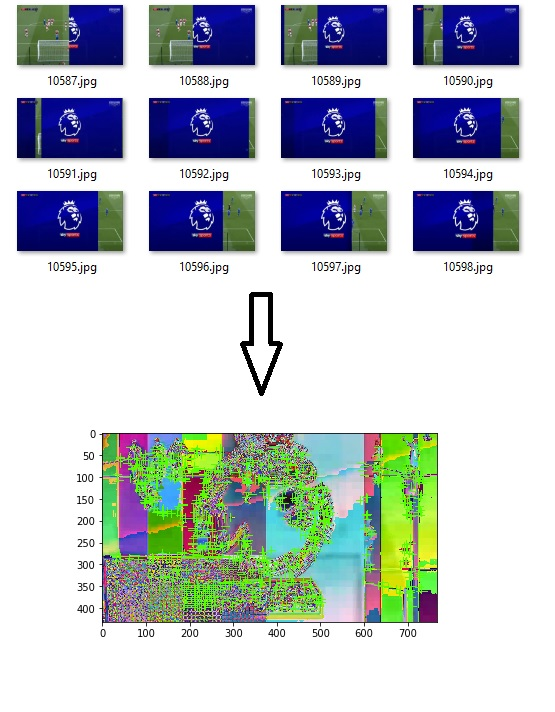
\includegraphics[width=.9\linewidth]{orb_window_diff_res.JPG}
\end{center}
\begin{verbatim}
- Récupérer W frames pour chaque shot, les régrouper en une fenêtre
  - nous obtenons |S| fenêtre de dimension W, où W est le nombre de frame
- Pour chaque fenêtre, calculer la matrice M égale à la différence de toute
  les autres frames dans la fenêtre
- Pour chaque matrice de différence, calculer ses features
  - nous obtenons |S| vecteur s
- Utiliser KMeans avec K=2 pour séparer les vecteurs en deux groupes
  - le groupe le plus petit est le groupe des logo
\end{verbatim}
Résultats :
De bons résultats sur la vidéo de PL.
Mauvais résultats sur les autres vidéos.

\subsection{Seconde approche : matching de contours}
\label{sec:orge885d02}
La méthode choisie différe avec les autres sur un point : au lieu de chercher à différencier les frames logo des frames non-logo, nous allons chercher les frames qui ont des formes en commun dans la vidéo.
En effet, d'après l'hypothèse III, il est fort probable que si un frame à l'instant t a beaucoup de formes en commun avec un frame à l'instant t', avec 2 < t' < 90 (hypothèse V), alors il y a un logo à l'instant t et un logo à l'instant t', et un replay entre t et '.
\subsubsection{Algorithme}
\label{sec:org46ef06d}
\begin{verbatim}
- Pré traitement sur les shots
  1. Redimensionner
  2. Cropper
  3. Supprimer le background (s’étendre la dessus)
  4. Détecter le contour (Canny Edge Detection)
  5. Génération des mosaiques
- Pour chaque mosaique de plan S_A :
  - Pour chaque mosaique de plan S_B après S_A :
    1. Contour_commun = C_A & C_B
    2. Contours_diff = Détection du contour de Contour_commun (cv2.findContours)
    3. Résultat = Ne garder que les contours qui sont assez longs (ceux qui ont au moins K points)
    4. Si Résultat > Seuil : alors S_A et S_B sont des logos potentiels
- Pour chaque logo potentiel LP :
  1. Le comparer avec les autres logo L’ (même procédure qu’en 2)
  2. Si au moins 2 logo L’  match, alors LP est un logo
- Trouver les replays grâce aux logos
\end{verbatim}
Pré traitement :
Les frames sont resizé puis cropé vers le centre (pour ne pas avoir l'affichage en haut de l'écran etc\ldots{}), puis un blur est appliqué (bilateralFilter, permet de filtrer certains faux positifs), et enfin on applique Canny Edge Detection.

Le point 3 de l’algorithme sert à filtrer les éventuels faux positifs.
Notre algorithme est sensible au plan fixe et aux images avec beaucoup de bruits (ces images ont beaucoup de contours détectés par l’algorithme de détection de contours).
Beaucoup de ces faux-positifs peuvent être filtrer lors du pré-traitement sur les plans, notamment en rajoutant du blur ou en supprimant le background, néanmoins, nous ne sommes pas parvenus à filtrer 100\% des faux-positifs.

\subsubsection{Mosaique de plan}
\label{sec:orgfcc85c9}
\subsubsection{{\bfseries\sffamily TODO} resize img + put them together ie A + B = C}
\label{sec:org7794fd1}
Pour chaque shot deux images au format .png (pas au format jpg, car celui-ci prend trop d'espace disque) sont générées.

Chaque image est de dimension I * I * width * height où I est le nombre de frame dans le shot.

Ces images sont en faites des matrices d'image qui vont permettre de comparer rapidement deux shot.
La première matrice a un décalage d'un frame par ligne, la seconde n'a pas de décalage.

Pour comparer deux shot, il suffit d’appliquer un ET binaire entre les matrices des mosaiques, puis de calculer la longueur du conteur dans cette matrice.
\begin{center}
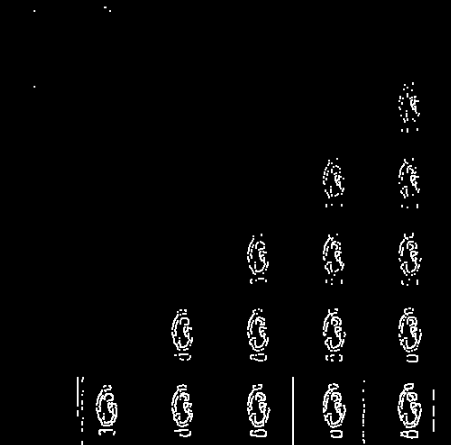
\includegraphics[width=.9\linewidth]{mosaique3.png}
\end{center}

\subsubsection{Résultats et limitation}
\label{sec:org8fd05b6}
Les résultats sans le filtrage des faux positifs (l’étape 3 de l’algorithme) sont un bon moyen d’évaluer l’efficacité de notre méthode.
\subsubsection{{\bfseries\sffamily TODO} : mettre les résultats ici}
\label{sec:org2e64dfe}
Concernant le temps d’exécution, celui-ci est relié presque entièrement à la taille de la vidéo donnée en entrée, ainsi qu’à la taille des mosaiques.

Les limitations de notre méthode sont les suivantes :
\begin{itemize}
\item Dans certaines vidéos, il n’y a pas de logo pour les replays (simple fondu)
\item Dans certaines vidéos, les logo de début et fin de replay ne sont pas les mêmes.
\item Dans certains vidéos, il y a des logo au début des replays, mais pas de logo à la fin des replays (un simple fondu remplace le logo).
\end{itemize}


\section{Apprentissage profond : les bases théoriques}
\label{sec:org5f19609}
Dans notre recherche, nous allons aborder plusieurs types de réseaux d'apprentissage automatique.
Nous allons présenter dans cette partie les principes fondamentaux à la bonne compréhension de ces derniers.

\subsection{Réseaux de neurones récurrents (RNN)}
\label{sec:org0c88cc6}
Les RNN (Recurrent Neural Networks), ou réseaux de neurones récurrents (RNR) en français, sont capables de répéter leur couche cachée, en utilisant comme entrée la sortie de toutes les couches précédentes et de générer une sortie pour chaque couche. 
Cela va leur permettre de prendre en entrée des séquences et de retourner des séquences.
En effet, pour une entrée [e\(_{\text{1}}\), e\(_{\text{2}}\),\ldots{}, e\(_{\text{n}}\)] et un initialiseur s\(_{\text{0}}\), le RNN va répéter n fois sa couche cachée, de telle sorte à générer une sortie s\(_{\text{1}}\) associée à la couche 1 et à l'entrée (e\(_{\text{1}}\), s\(_{\text{0}}\)); puis il va générer une sortie s\(_{\text{2}}\) associée à la couche 2 et à l'entrée (e\(_{\text{2}}\), s\(_{\text{1}}\)), etc \ldots{}
Pour finir, nous aurons en sortie la séquence [s\(_{\text{1}}\), s\(_{\text{2}}\), \ldots{}, s\(_{\text{n}}\)].

Par exemple, appliqués à la génération de phrase, les RNN vont être capables de générer (mot par mot, ou n-gram par n-gram) des séquences de phrases de longueur arbitraire.

Pour apprendre un modèle, le RNN va avoir besoin d'un ensemble d'entraînement qui met en avant les propriétés qui nous intéressent dans le modèle.

La nature récursive de ces réseaux les rend particulièrement adaptés aux tâches de traitement du langage naturel.

\subsection{LSTM}
\label{sec:orgedcdbad}
Les LSTM (Long Short Term Memory) sont un type de RNN \textbf{à portes (gated RNN)}. Ces réseaux sont sur l'unité récurrente à portes. 
Ces portes vont permettre de stocker l'information apprise par le réseau à travers le temps. 
À la différence des RNN classiques, les LSTM sont capables d'oublier de l'information grâce à leur \textbf{leaky unit} afin d'éviter une explosion ou une disparition du gradient.
Concrétement, cela va leur permettre de pouvoir capturer des dépendances à long terme de manière bien plus efficace que les RNN classiques.

\subsection{CNN}
\label{sec:org55300c2}
Les CNN (Convolutional Neural Networks), ou réseaux de neurones convolutifs (RNC) en français, sont un type de réseau de neurones qui utilisent la convolution au lieu de la multiplication matricielle dans au moins une de leurs couches.
La convolution est une opération qui prend en argument l'entrée (typiquement un vecteur représentant une donnée) et un \textbf{noyau} (les paramètres qui vont être appris par le CNN) et renvoie une \textbf{carte de caractéristiques} (feature map).
Le noyau est une matrice qui va parcourir l'entrée et appliquer l'opération de convolution. 
Pour parcourir l'entrée, celle-ci va être divisée en plusieurs matrices carrées de même taille que le noyau (par ex 2x2 ou 6x6) en ajouteur si nécessaire du \emph{padding} et du \emph{striding}.
La fonction de convolution a trois caractéristiques importantes : l'\textbf{intéraction parcimonieuse} ("sparse interaction"), le \textbf{partage de paramètres} et les \textbf{représentations équivariantes}.
La couche de convolution est généralement composée de la fonction de convolution suivie d'une fonction d'activation non linéaire (par exemple, ReLU ou tanh) et d'une d'une fonction de \textbf{pooling}.

\subsubsection{Intéraction parcimonieuse}
\label{sec:org75f3c5a}
\begin{center}
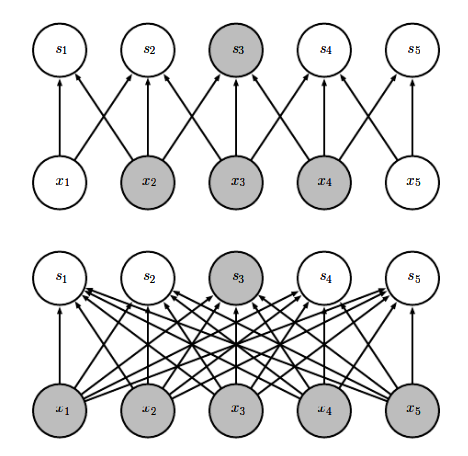
\includegraphics[width=.9\linewidth]{sparse_vs_dense.png}
\end{center}
À la différence des réseaux classiques où toutes les entrées intéragissent avec toutes les entrées, les réseaux à convolution ont des \textbf{intéractions parcimonieuses}. 
C'est à dire que la taille du noyau (donc de l'intéraction avec l'entrée), est plus petite que la taille de l'entrée.
C'est pourquoi les réseaux à convolution sont très efficaces pour le traitement d'image.
En effet, une image a une dimension en entrée de \emph{c*l*w} où \emph{c} est le nombre de canaux de l'image (un seul pour une image en noir et blanc, trois pour une image en couleur), l la largeur en pixel de l'image et w la longueur en pixel de l'image.
Une peite image couleur de dimension 100*100 aura 100*100*3 paramètres en entrée, ce qui provoque une explosion combinatoire avec les réseaux classiques qui n'ont pas d'intéraction parcimonieuse.
Un réseau de convolution, quant à lui, aura un noyau d'une dizaine ou d'une centaine de pixel qui parcourt l'image à la recherche de caractéristiques significatives comme des contours.
Ils ont besoin de stocker moins de paramètres, ils ont donc ont besoin de moins de mémoire (pour la même tâche) et ont une meilleure efficacité statistique.

\subsubsection{Partage de paramètres}
\label{sec:orgbaf791b}
Dans un réseau classique, un poid (un paramètre) est associé à chaque paramètre d'entré et ne sert qu'une fois.
Tandis que dans un réseau convolutif, le noyau utilisé par une couche de convolution est le même sur toutes les matrices représentant l'entrée. 
Grâce à ce \textbf{partage des paramètres}, il n'y a qu'un les poids du noyau à apprendre au lieu d'un poid pour chaque neurone d'entrée.
De plus, la taille du noyau est en général largement inférieure à celle de la couche d'entrée.

\subsubsection{Représentations équivariantes}
\label{sec:orgcc3b14a}
Une fonction est \textbf{équivariante} si, quand l'entrée change, la sortie change de la même manière.
En terme mathématique, cela signifique que si \(y = f(x)\) alors \(g(y) = g(f(x))\). 
Les réseaux convolutifs sont équivariants à la translation. 
Dans le cas de l'image, celà signifie que le déplacement des pixels n'a pas d'influence sur le réseau.

\subsubsection{Pooling}
\label{sec:org3f15550}
La fonction de pooling va modifier la sortie de la couche de convolution.
Pour chaque valeur dans la carte des caractéristiques à la sortie de la convolution (après la fonction d'activation), la fonction de pooling va remplacer celle-ci en fonction de la valeur des cases voisines dans la carte.
Une fonction de pooling usuelle est max pooling, qui va renvoyer la plus grande valeur dans un voisinage rectangulaire.
L'utilité de la fonction de pooling est de rendre la représentation apprise par la couche de convolution \textbf{invariante} à de petites modifications sur l'entrée.
Par exemple, dans le cas de la reconnaissance d'image, le réseau ne va pas chercher dans l'image en entrée les informations au pixel près.
Si le réseau a appris à détecter les visages, il n'a pas besoin de retrouver l'emplacement des yeux au pixel près, une position approximative de ceux-ci lui suffira.
Une autre utilité du pooling est de réduire la taille de la sortie de la couche de convolution.
Nous pouvons voir le pooling comme un résumé de la carte des caractéristiques obtenue par convolution.

\section{Apprentissage profond : état de l'art pour la reconnaissance d'action dans les vidéos}
\label{sec:orgc62ba9f}
Nous nous intéressons à l'état de l'art concernant la détection d'action dans les vidéos. 
En effet, la transition d'un logo s'effectue sur plusieurs frames consécutives; il y a donc une composante temporelle à notre recherche, et nous pouvons considérer la transition d'un logo comme une action.

\subsection{Two-Stream Convolutional Networks for Action Recognition in Videos}
\label{sec:org7704dbb}
Cet article est écrit par Karen Simonyan et Andrew Zisserman. Dans celui-ci, ils proposent de séparer la tâche de reconnaissance d'action dans les vidéos en deux parties : une composante spatiale et une composante temporelle.
La composante spatiale contient l'information concernant sur les objets dans la vidéo; tandis que la composante temporelle l'information sur les déplacements de ces objets et de la caméra.
A partir de ces observations, les auteurs proposent d'entraîner un classifieur spatial (Spatial stream ConvNet) et un classifieur temporel (Temporal stream ConvNet).
Ces classifieurs sont des réseaux de neurones convolutifs profonds.

\subsubsection{Classifieur spatial}
\label{sec:org351c09e}
Ce réseau a une architecture de classifieur d'image classique. 
Il va permettre de donner un indice fort pour la prédiction, car certaines actions sont très liées à certains objets.
De plus, la recherche dans le domaine de la classification est un domaine à part entière;
toutes les avancées dans le domaine augmenteront l'efficacité de ce classifieur.
Il n'est pas nécessaire d'apprendre ce réseau "from scratch" (de zéro), les approches de transfer learning sont efficaces.

\subsubsection{Classifieur temporel}
\label{sec:orgb5c3e45}
\begin{center}
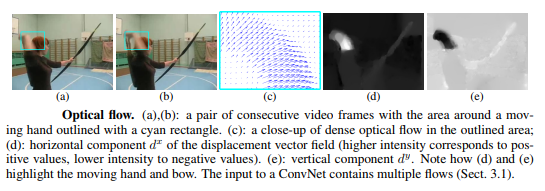
\includegraphics[width=.9\linewidth]{optical_flow.png}
\end{center}
Source : Two-Stream Convolutional Networks for Action Recognition in Videos, Figure 2
L'innovation de l'article vient de l'introduction du classifieur temporel.
L'idée est de détecter le mouvement des objets dans la vidéo, car un mouvement est la représentation d'un objet dans le temps.
Les auteurs appellent leur approche "optical flow stacking" (empilement de flux optique).
Dans celle-ci, ils utilisent la méthode "optical flow" pour détecter le mouvement des objets entre des frames consécutives.
Ils définissent aussi un hyperparamètre L qui définit la distance maximum entre deux frames pour laquel il faut calculer le flux optique.
Par exemple, si L=5, alors pour le frame t, il faudra calculer le flux entre le frame t et le frame t+1; entre t+1 et t+2; etc\ldots{} jusqu'à t+4 à t+5.
Chacun de ces flux servira d'entrée au classifieur temporel pour le frame t.

\subsubsection{Méthode d'évalutation et résultats obtenus}
\label{sec:org6b8f7b5}
\begin{center}
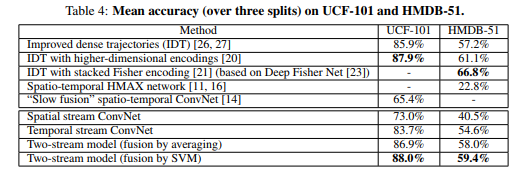
\includegraphics[width=.9\linewidth]{two_stream_res.png}
\end{center}
Source : Table 4: Mean accuracy (over three splits) on UCF-101 and HMDB-51.

Le classifieur spatial est pré-entrainé avec ImageNet, tandis que le temporel
est entraîné de zéro (car il n'y a pas de réseau déjà entraîné pour cette tâche).
Les dataset utilisés pour l'entraînement et l'évaluation sont UCF-101 et HMDB-51,
contenant à eux deux près de 20000 vidéos annotées.

\textbf{Note} Pour calculer la classe d'un frame à l'instant t, les auteurs proposent
deux méthodes :
\begin{itemize}
\item fusion par la moyenne (by averaging) : y\(_{\text{t}}\) = y\(_{\text{t}}\)\(_{\text{spatial}}\) + y\(_{\text{t}}\)\(_{\text{temporal}}\) / 2
\item fusion par SVM (by SVM) : un SVM multiclasse linéaire est entrainé pour
\end{itemize}
prédire la classe à partir du softmax des scores L2-normalisés.

Les résultats en \textbf{link table} montrent l'efficacité de leur méthode par rapport
aux autres approches état de l'art.

Nous pouvons voir que leur approche two-stream avec fusion SVM est la plus
efficace sur le dataset UCF-101, et qu'elle a aussi de bons résultats sur
HMDB-51.

Ce qui est le plus intéressant dans cet article, c'est l'amélioration
qu'apporte l'ajout de la composante temporelle.
En effet, le classifieur d'image simple (spatial) n'a que 73.0\% (UCF-101) et 40.5\% (HMBD-51), tandis que le classifieur qui prend en compte l'image et la temporalité (two-stream model) atteint \textbf{88.0\%} et 59.4\%; ce qui est une nette amélioration.
Cet article nous a renforcé dans l'hypothèse qu'il est nécessaire d'étudier une vidéo non pas comme une suite d'image indépendante, mais comme une suite de séquence avec un lien au sein de chaque séquence.
Il semblerai que la temporalité a une très grande importance pour  l'analyse de vidéos.

\subsection{Learning Spatiotemporal Features with 3D Convolutional Networks}
\label{sec:orgdf5c403}

Dans cet article, Du Tran et. al proposent une approche pour apprendre les caractéristiques spatio-temporelles dans les vidéos grâce à un réseau de neuronnes profond.
L'objectif est d'apprendre des caractéristiques qui soient :
\begin{itemize}
\item générique : c'est à dire la capacité à representer différents types de vidéos
\item compact : afin de pouvoir stocker un grand nombre de ces caractéristiques
\item efficace (computationnellement): pour traiter les vidéos en temps réel
\item simple (à implémenter) : afin de fonctionner même avec les modèles simples (comme un classifieur linéaire)
\end{itemize}

\subsubsection{Apport de l'article}
\label{sec:org6e71902}
\begin{center}
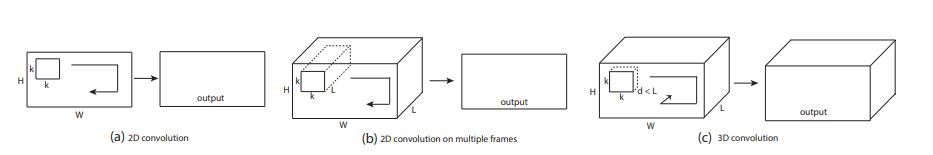
\includegraphics[width=.9\linewidth]{3D_vs_2_stream.JPG}
\end{center}
Source : Learning Spatiotemporal Features with 3D Convolutional Networks Figure 1
Dans l'approche Two-Stream Convolutional Networks for Action Recognition in Videos \cite{DBLP:journals/corr/SimonyanZ14}, deux réseaux à convolution 2D sont utilisés (un spatial et un temporel).
L'apprentissage du réseau temporel est séparé de celui du réseau réseau spatial, ce qui ne permet pas d'avoir un réseau capturant l'information temporel relativement à l'information spatial.
De plus, même si le réseau temporel prend plusieurs frames en entrée (paramètre L > 1), la convolution 2D va écraser la composante temporelle car sa sortie sera une image (2D).
La figure \textbf{XXX} illustre la différence entre un réseau à convolution 2D (approche de K. Simonyan et A. Zisserman) et un réseau à convolution 3D (Tran et al.). Un réseau à convolution 2D aura en sortie une image (2D) même si l'entrée est une séquence d'images, tandis qu'un réseau à convolution 3D aura en sortie une image relative à une autre dimension (dans notre cas, le temps).

En choisissant d'entraîner leur réseau à partir de séquence d'images, les auteurs espèrent pouvoir apprendre la temporalité d'une manière "moins artificielle" que dans l'approche précédente (qui nécessite un pré-traitement sur les images pour pouvoir calculer les images d'optical flow servant au réseau temporel).

\subsubsection{Architecture et entraînement du réseau}
\label{sec:org4862e0f}
\begin{center}
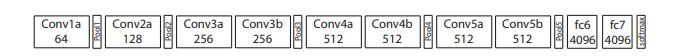
\includegraphics[width=.9\linewidth]{c3d_architecture.jpg}
\end{center}
Source : Figure 3
L'entrée de ce réseau est de dimension c * l * h * w où c est le nombre de canal des images (3 pour la couleur, 1 pour les images en noir et blanc), l le nombre d'image dans les séquences, h la longueur et w la largeur.
L'architecture conseillée par les auteurs est 8 couches de convolution et 5 couches de pooling, ainsi que 2 couches complètement connectées et la fonction softmax pour la couche de sortie.
Le kernel recommandé par les auteurs est 3 * 3 * 3 avec un pas (stride) de 1 * 1 * 1 pour toutes les couches de convolution.
Toutes les couches de pooling sont max pooling avec une taille de kernel 2 * 2 * 2 (sauf pour la première qui est 1 * 2 * 2) avec un stride 2 * 2 * 2 (sauf pour la première qui a un stride de 1 * 2 * 2).
Pour finir avec l'architecture, les deux couches complètement connectées ont 4096 sorties.

Ce réseau va être entraîné de zéro par descente du gradient à partir de séquences d'images annotées.
Le taux d'apprentissage est de 0.003 et est divisé par 10 toutes les 4 epoch.
L'entraînement s'arrête après 16 epoch.

Après l'entraînement, le réseau peut être utilisé comme un extracteur de caractéristique pour des tâches d'analyse vidéo.
Pour se faire, la vidéo va être découpée en des clips de 16 frames (avec 8 frames de chevauchement entre deux clips consécutifs).
Ensuite, chacun de ces clips va être passé au réseau et l'avant dernière couche complètement connectée (fc6) va contenir les caractéristisques du clip.

\textbf{Qu'est-ce que ce réseau apprend ?} Ce réseau apprend à se focalisant sur l'image des premiers frames, et à traquer leur déplacement dans les frames suivants.

\subsubsection{Résultat pour la tâche de reconnaissance d'action}
\label{sec:org9a1f928}
\begin{center}
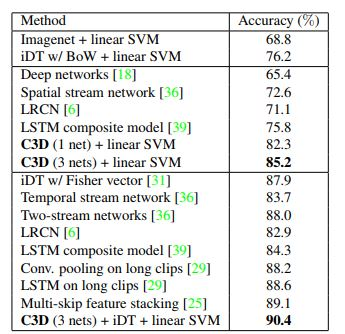
\includegraphics[width=.9\linewidth]{c3d_result.jpg}
\end{center}
Ces résultats ont été obtenus par les auteurs pour la tâche de reconnaissance d'action sur le corpus de vidéo UCF101.
Nous voyons que l'approche par réseau à convolution 3D est la plus efficace.

\subsubsection{Conclusion}
\label{sec:orgb9605f9}
Dans cet article, les auteurs ont adressé le problème de la temporalité dans les vidéos.
Ils ont montré qu'un réseau à convolution 3D est capable de modéliser l'information temporelle et spatiale simultanément, et donc d'obtenir de meilleurs résultats que les réseaux à convolution 2D sur plusieurs tâches d'analyse de vidéos.
Pour ma part, je trouve cette approche très intéressante et élégante, de par sa simplicité.
En effet, le réseau apprend la temporalité sans qu'il soit nécessaire d'injecter l'information temporelle de manière artificielle ou bien en compliquant l'architecture du réseau.

\subsection{Beyond Short Snippets: Deep Networks for Video Classification}
\label{sec:orgf550b49}
Dans cet article \cite{Joe_Yue_Hei_Ng_2015}, les auteurs proposent d'utiliser une architecture hybride à base de CNN et de RNN (LSTM) pour l'analyse vidéo.
Les CNN sont des réseaux particulièrement efficaces pour analyser les frames des vidéos, c'est le CNN qui va se charger de la composante spatiale de la vidéo.

\begin{center}
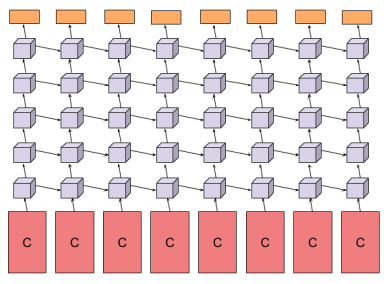
\includegraphics[width=.9\linewidth]{cnn_lstm.PNG}
\end{center}
Source : Beyond Short Snippets: Deep Networks for Video Classification; Figure 3
\subsubsection{Approche}
\label{sec:orga290ccb}
L'aspect le plus important de la recherche des auteurs concernent la manière dont le LSTM va recevoir l'information du CNN.
Deux architectures de CNN sont utilisés par les auteurs : AlexNet et GoogLeNet.
Afin que le LSTM puisse utiliser la sortie du CNN, il est nécessaire d'avoir une architecture de pooling efficace.
Les auteurs en proposent cinq.

\section{Collecte des données pour l'apprentissage profond}
\label{sec:org7e77240}
L'approche par matching de contours convient tout à fait à la tâche de scrapping.
En effet, elle est :
\begin{itemize}
\item rapide : moins de \textbf{X} minutes sur une machine \textbf{machine de référence EC2 (ou autre)} pour une vidéo de 90 minutes à 60 fps
\item précise : seulement \textbf{X} \% de faux positifs sur \textbf{Y} logos scrappés
\end{itemize}

\subsubsection{Architecture du scrapper}
\label{sec:orgb0d3535}
\begin{itemize}
\item requête HTTP avec une ID youtube => logo uploadé sur GCP
\item image docker (avec le serveur à l'écoute des requêtes) déployée sur le cloud
\end{itemize}
Cette architecture est scalaire; ceci nous a permi de scrapper plusieurs vidéos en parallèle et d'obtenir un dataset conséquent.

\subsection{Datasets}
\label{sec:org889af4e}
\begin{itemize}
\item Dataset non logo
\item Dataset logo
\item Dataset logo séparé en fonction du logo (ligue 1, premier league, \ldots{})
\end{itemize}


\subsection{Détection des frames logo}
\label{sec:orgbc47042}
\subsubsection{Propre modèle}
\label{sec:org34b0835}
\subsubsection{VGG net}
\label{sec:orga1c711f}
\subsubsection{Transfert Learning}
\label{sec:org20ecd3d}
\subsubsection{Comparaison résultat}
\label{sec:orga2d0f90}

\subsection{Détection des séquences de frames logo}
\label{sec:orgd5217e2}

\section{Appendice}
\label{sec:org8961bc3}
Clustering : procédé permettant de regrouper des éléments
Histogramme : représentation d'une image en fonction de ses canaux de couleurs (rouge, vert, bleu)
Frame : une image à l'instant t d'une vidéo
Shot : un plan
FPS : frame per second / image par seconde
Cropper : sélectionner une partie continue des pixels l'image
RNN : Recurrent Neural Networks, ou réseaux de neurones récurrents (RNR) en français
CNN : Convolutional Neural Network, réseaux de neurones convolutifs (RNC) en français
LSTM : Long Short Term Memory

\section{Bibliographie}
\label{sec:org534b7aa}
\subsection{Articles relatifs à l'apprentissage profond}
\label{sec:orgd7f1756}
Gradient-Based Learning Applied to Document Recognition; Y. LeCun, L. Bottou, Y. Bengio, P. Haffner; 1998
Learning Hierarchical Features for Scene Labeling; C. Farabet, C. Couprie, L. Y. LeCun; 2013
Two-Stream Convolutional Networks for Action Recognition in Videos; K. Simonyan, A. Zisserman; 2014
Learning Spatiotemporal Features with 3D Convolutional Networks; D. Tran, L. Bourdev; R. Fergus; L. Torresani; M. Paluri; 2014
Beyond Short Snippets: Deep Networks for Video Classification; J.Y.H. Ng, M. Hausknecht; 2015
L'apprentissage profond; I. Goodfellow, Y. Bengio, A. Courville ; 2015
\subsection{Articles relatifs à la détection de replays}
\label{sec:org03ba4d5}
A Robust Replay Detection Algorithm for Soccer Video; W. Xu, Y. Yi(2011).
Replay and key-events detection for sports video summarization using confined elliptical local ternary patterns and extreme learning machine; A. Javed, A. Irtaza; 2019
Video Co-summarization: Video Summarization by Visual Co-occurrence; W. Chu; 2015
\ref{pan} Automatic Detection Of Replay Segments In Broadcast Sports Programs By Detection Of Logos In Scene Transitions; H. Pan; 2002
Mean Shift Based Video Segment Representation And Applications To Replay Detection; L. Duan; 2004
Online, Simultaneous Shot Boundary Detection And Key Frame Extraction For Sports Videos Using Rank Tracing; W. Abd-Almageed; ‎2008
On-line Key Frame Extraction and Video Boundary Detection using Mixed Scales Wavelets and SVD; A. Azeroual; 2016
Highlight Summarization in Soccer Video based on Goalmouth Detection; Z. Zhao; 2006
A General Framework for Automatic On-line Replay Detection in Sports Video; B. Han, Y. Yan; 2009
An Efficient Framework for Automatic Highlights Generation from Sports Videos; A. Javed; 2016
A New Slow-Motion Replay Extractor For Soccer Game Videos; E. Farn, L. Chen; 2003
Fast Highlight Detection and Scoring for Broadcast Soccer Video Summarization using On-Demand Feature Extraction and Fuzzy Inference; M. Sigari, H. Soltanian-Zadeh;  2015
Automatic Summarization Of Soccer Highlights Using Audio‑visual Descriptors; A. Raventós, R. Quijada, L. Torres, F. Tarrés; 2014
A Novel Method For Slow Motion Replay Detection In Broadcast Basketball Video; C. Chen; 2014

\subsection{Articles générals de vision par ordinateur}
\label{sec:org03a4bbb}
ORB: an efficient alternative to SIFT or SURF; E. Rublee, V. Rabaud; 2011

\section{Table des figures}
\label{sec:org6441457}
\ref{calc-dist} Xu, W., \& Yi, Y. (2011). A Robust Replay Detection Algorithm for Soccer Video. IEEE Signal Processing Letters, 18(9). Equation (4)
\ref{sparse-vs-dense} I. Goodfellow, Y. Bengio, A. Courville ; L'apprentissage profond; 2015; Chapitre 9, Figure 9.2

\bibliographystyle{unsrt}
\bibliography{summary}
\end{document}
